\subsection{Flyvehøjde}

Dette afsnit beskriver test af tilpasning af flyvehøjde.

For at dronen ved hvilken højde den skal flyve i, skal flyveopsætningen være hentet fra serveren. Når flyvehøjden og de ønskede GPS positioner er kendt, begynder dronen at lette. Main controlleren anvender højdesensorer til at finde højden med. Så længe at højden ikke er indenfor det ønskede interval, skal den hæve eller sænke sin højde, det gør den ved enten at forøge eller formindske throttle. 

På figur \ref{fig:skift_hoejde} ses hvad der sker, hvis højden enten er for høj eller for lav. Først måles den aktuelle højde, denne sammenlignes med minimums- og maksimalhøjde, hvis den er udenfor intervallet reguleres der på throttle. 
På figur \ref{fig:skift_hoejde} er der vist to scenarier, et hvor højden er for lav og et hvor højden er for høj.

\begin{figure}[H]
\centering
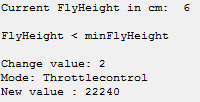
\includegraphics[width=0.5\textwidth]{Billeder/Test/skift_hoejde.png}
\caption{Tilpasning af højde}
\label{fig:skift_hoejde}
\end{figure}

Når højden er i intervallet, vil den stadig reguleres. Dette foregår i mindre steps af gangen, og det sikrer at den holder sig stabil.
Figur \ref{fig:interval_skift} viser hvad den aktuelle højde er og hvor meget den er skiftet siden sidste måling. Udefra dette reguleres højden, hvis forskellen er positiv, vil den forsøge at gå ned i højde.

\begin{figure}[H]
\centering
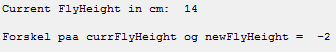
\includegraphics[width=0.6\textwidth]{Billeder/Test/hoejdei_interval_skift.png}
\caption{Interval højde skift}
\label{fig:interval_skift}
\end{figure}